\documentclass{beamer}
\usepackage{graphicx}
\usepackage{amsmath, esint}

\usepackage{ragged2e}
\usepackage{tikz}
\usetikzlibrary{arrows,shapes}

\usepackage{listings}
\lstset{escapeinside={@(}{)@}}
\usepackage{algorithm}
\usepackage{algorithmic}

\usepackage{tabularx}
\newcolumntype{Y}{>{\centering\arraybackslash}X}

\usepackage{minted}
\usepackage{xcolor} 
\definecolor{LightGray}{gray}{0.975}

\usepackage{amssymb}

\def\ojoin{\setbox0=\hbox{$\bowtie$}%
  \rule[-.02ex]{.25em}{.4pt}\llap{\rule[\ht0]{.25em}{.4pt}}}
\def\leftouterjoin{\mathbin{\ojoin\mkern-5.8mu\bowtie}}
\def\rightouterjoin{\mathbin{\bowtie\mkern-5.8mu\ojoin}}
\def\fullouterjoin{\mathbin{\ojoin\mkern-5.8mu\bowtie\mkern-5.8mu\ojoin}}

%\usetheme{Warsaw}
\usefonttheme{serif} 

\title[Chapter 17]{Database System Concepts, $7^{th}$ Edition \\ Chapter 17: Transactions}
\author{Silberschatz, Korth and Sudarshan}
\date{\today}

\setbeamertemplate{navigation symbols}{}%remove navigation symbols

\defbeamertemplate*{footline}{shadow theme}
{%
  \leavevmode%
  \hbox{\begin{beamercolorbox}[wd=.5\paperwidth,ht=2.5ex,dp=1.125ex,leftskip=.3cm plus1fil,rightskip=.3cm]{author in head/foot}%
    \usebeamerfont{author in head/foot} Database System Concepts \hfill \insertshorttitle
  \end{beamercolorbox}%
  \begin{beamercolorbox}[wd=.5\paperwidth,ht=2.5ex,dp=1.125ex,leftskip=.3cm,rightskip=.3cm plus1fil]{title in head/foot}%
    \usebeamerfont{title in head/foot} \hfill \insertframenumber\,/\,\inserttotalframenumber%
  \end{beamercolorbox}}%
  \vskip0pt%
}

\AtBeginSection[]
{
     \begin{frame}<beamer>
     \frametitle{Plan}
     \tableofcontents[currentsection]
     \end{frame}
}

\newcommand{\toRight}[1]{
    \begin{FlushRight}
        {\tiny #1}
    \end{FlushRight}
} % Align to right

\begin{document}

\frame{\titlepage}

\begin{frame}{Database System Concepts}
    \centering
    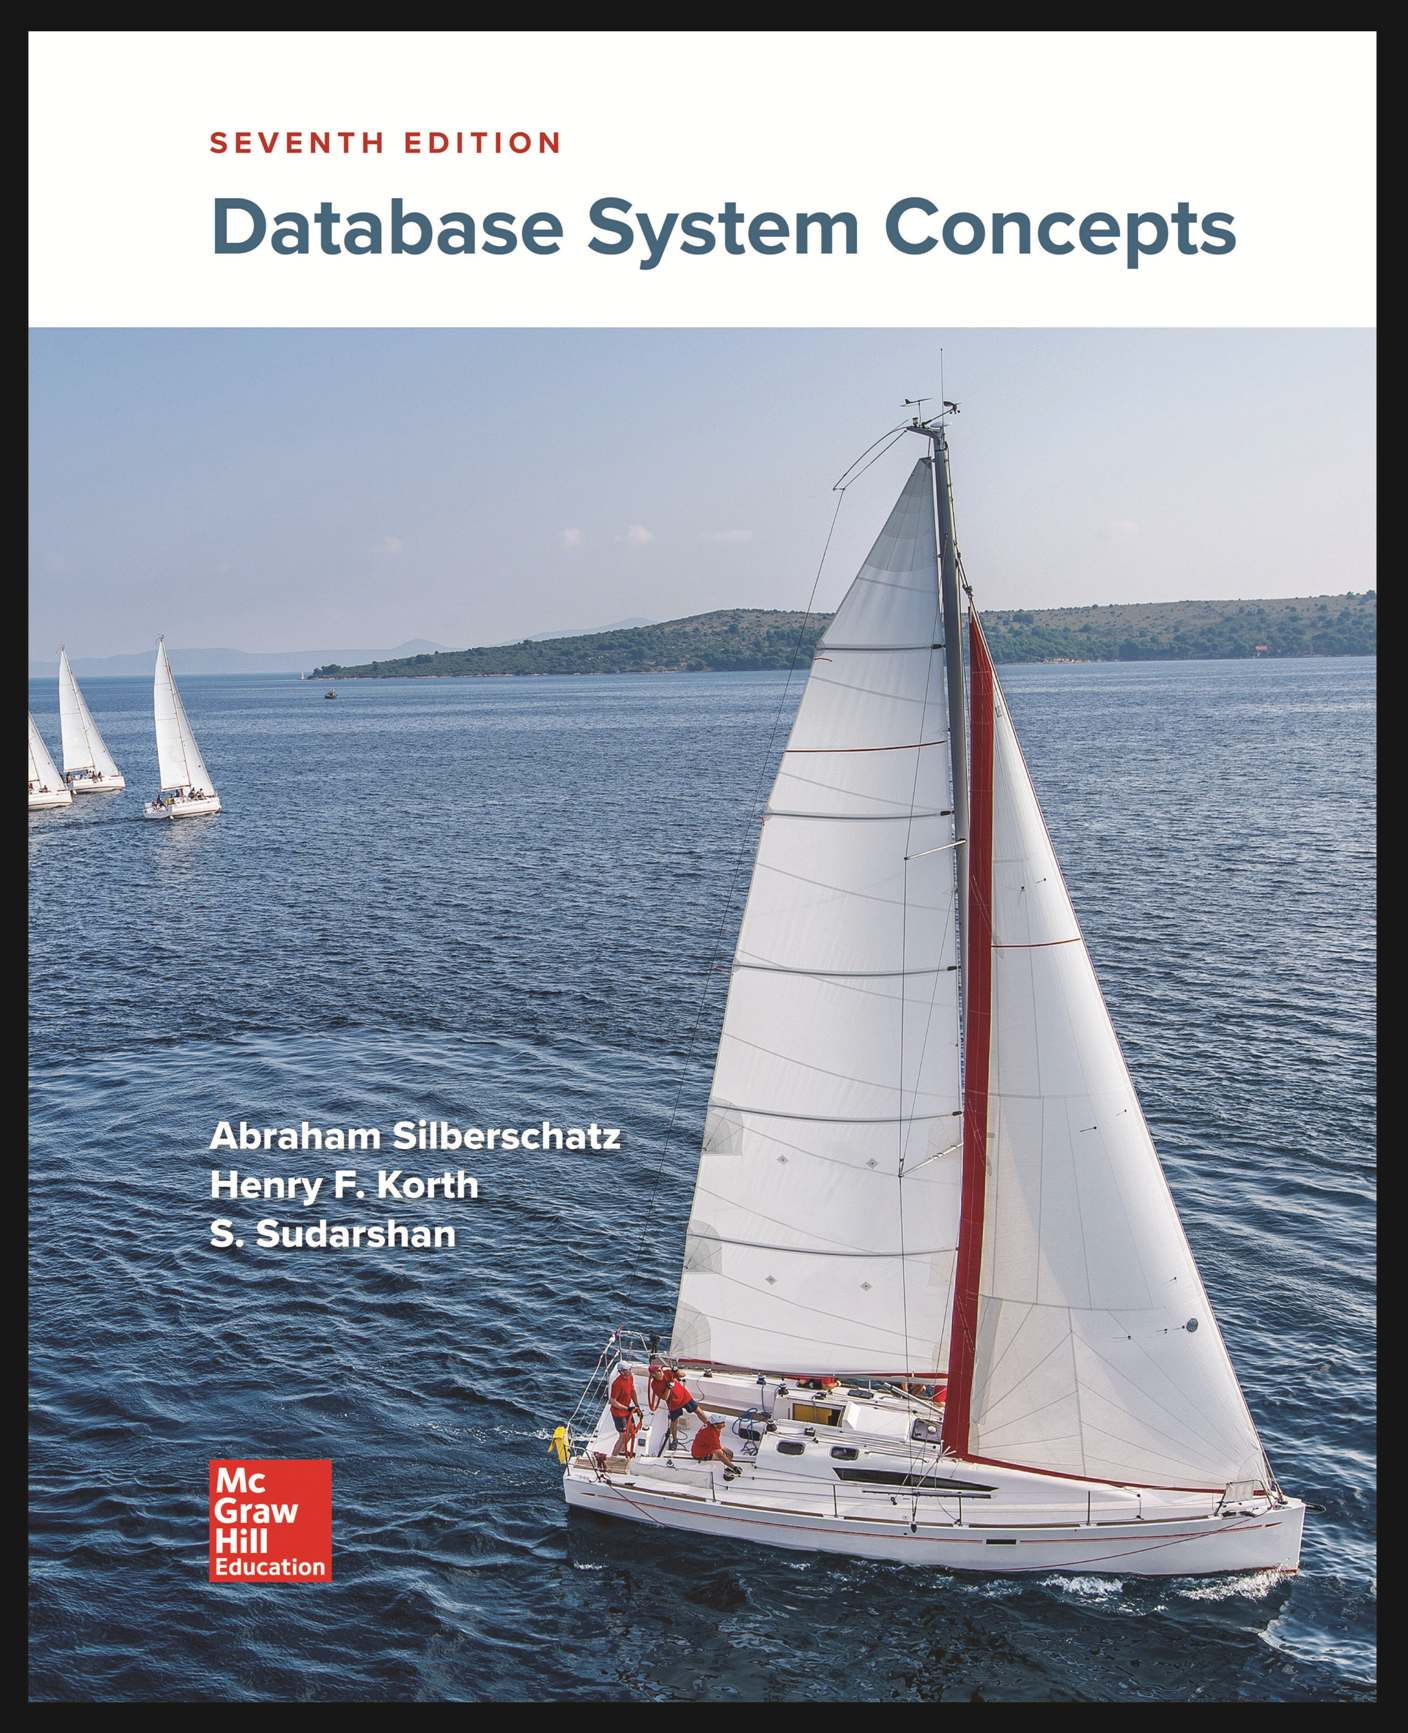
\includegraphics[width=0.5\textwidth]{figures/book_cover.jpg} \\
    \vspace{5mm}
    {
        \tiny
        Content has been extracted from \textit{Database System Concepts}, Seventh Edition, by Silberschatz, Korth and Sudarshan. Mc Graw Hill Education. 2019.\\
        Visit \url{https://db-book.com/}.\\
    }
\end{frame}

\section{Transaction Concept}

\begin{frame}{Transaction Concept}
    A \textbf{transaction} is a unit of program execution that accesses and possibly updates various data items.
    \begin{itemize}
        \item Example of a simple transaction to transfer \$50 from account A to account B:
        \begin{enumerate}
            \item \texttt{read(A)}
            \item \texttt{A := A - 50}
            \item \texttt{write(A)}
            \item \texttt{read(B)}
            \item \texttt{B := B + 50}
            \item \texttt{write(B)}
        \end{enumerate}
        \item Two main issues to deal with:
        \begin{itemize}
            \item Failures of various kinds, such as hardware failures and system crashes
            \item Concurrent execution of multiple transactions
        \end{itemize}
    \end{itemize}
\end{frame}

\begin{frame}{Example of Fund Transfer}
    \scriptsize
    Transaction to transfer \$50 from account A to account B:
    \begin{enumerate}
        \item \texttt{read(A)}
        \item \texttt{A := A - 50}
        \item \texttt{write(A)}
        \item \texttt{read(B)}
        \item \texttt{B := B + 50}
        \item \texttt{write(B)}
    \end{enumerate}

    \textbf{Atomicity Requirement}
    \begin{itemize}
        \item Transactions must be atomic - either all operations are executed or none are.
        \item Example:
        \begin{enumerate}
            \scriptsize
            \item If a failure occurs after writing A but before writing B, the system must roll back to a consistent state.
            \item Ensures no partial transactions are committed.
        \end{enumerate}
    \end{itemize}

    \textbf{Durability Requirement}
    \begin{itemize}
        \item Once the user has been notified that the transaction has completed (i.e., the transfer of the \$50 has taken place), the updates to the database by the transaction must persist even if there are software or hardware failures.
    \end{itemize}

\end{frame}

\begin{frame}{Example of Fund Transfer (Cont.)}

    \scriptsize
    \textbf{Consistency Requirement}
    \begin{itemize}
        \item The database must remain in a consistent state before and after a transaction.
        \item The sum of A and B is unchanged by the execution of the transaction.
        \item Example:
        \begin{itemize}
            \scriptsize
            \item If a transaction debits one account and credits another, the total balance must remain the same.
        \end{itemize}
        \item In general, consistency requirements include
            \begin{itemize}
                \scriptsize
                \item Explicitly specified integrity constraints such as primary keys and foreign keys
                \item Implicit integrity constraints.
                \item A transaction must see a consistent database.
                \item During transaction execution the database may be temporarily inconsistent.
                \item When the transaction completes successfully the database must be consistent. Erroneous transaction logic can lead to inconsistency
            \end{itemize}
    \end{itemize}

\end{frame}

\begin{frame}{Example of Fund Transfer (Cont.)}

    \scriptsize
    \textbf{Isolation Requirement}
    \begin{itemize}
        \item if between steps 3 and 6, another transaction T2 is allowed to access the partially updated database, it will see an inconsistent database (the sum A + B will be less than it should be).
            \begin{tabular}{l l}
                \textbf{T1}                 & \textbf{T2} \\
                1. \texttt{read(A)}         &       \\
                2. \texttt{A := A - 50}     &       \\
                3. \texttt{write(A)}        &       \\
                                            &   \texttt{read(A), read(B), print(A+B)} \\
                4. \texttt{read(B)}         &       \\
                5. \texttt{B := B + 50}     &       \\
                6. \texttt{write(B)}        &       \\
            \end{tabular}

        \item Isolation can be ensured trivially by running transactions \textbf{serially}.  That is, one after the other.
        \item However, executing multiple transactions concurrently has significant benefits, as we will see later.
        \item Each transaction should appear as if it executes in isolation.
        \item Intermediate states must not be visible to other transactions.

    \end{itemize}
\end{frame}

\begin{frame}{ACID Properties}

    \scriptsize
    A \textbf{transaction} is a unit of program execution that accesses and possibly updates various data items.To preserve the integrity of data the database system must ensure:
        \begin{itemize}
            \item \textbf{Atomicity}. Either all operations of the transaction are properly reflected in the database or none are.
            \item \textbf{Consistency}. Execution of a transaction in isolation preserves the consistency of the database.
            \item \textbf{Isolation}. Although multiple transactions may execute concurrently, each transaction must be unaware of other concurrently executing transactions. Intermediate transaction results must be hidden from other concurrently executed transactions.
                \begin{itemize}
                    \scriptsize
                    \item That is, for every pair of transactions $T_i$ and $T_j$, it appears to $T_i$ that either $T_j$, finished execution before $T_i$ started, or $T_j$ started execution after $T_i$ finished.
                \end{itemize}
            \item \textbf{Durability}. After a transaction completes successfully, the changes it has made to the database persist, even if there are system failures.
        \end{itemize}

\end{frame}

\section{Transaction State}

\begin{frame}{Transaction States}
    Transactions progress through several states:
    \begin{itemize}
        \item \textbf{Active} - the initial state; the transaction stays in this state while it is executing.
        \item \textbf{Partially Committed} - after the final statement has been executed.
        \item \textbf{Failed} - after the discovery that normal execution can no longer proceed.
        \item \textbf{Aborted} - after the transaction has been rolled back and the database restored to its state prior to the start of the transaction. Two options after it has been aborted.  Rolled back, possibly restarted.
        \item \textbf{Committed} - after successful completion.
    \end{itemize}
\end{frame}

\begin{frame}{Transaction States (Cont.)}
    \centering
    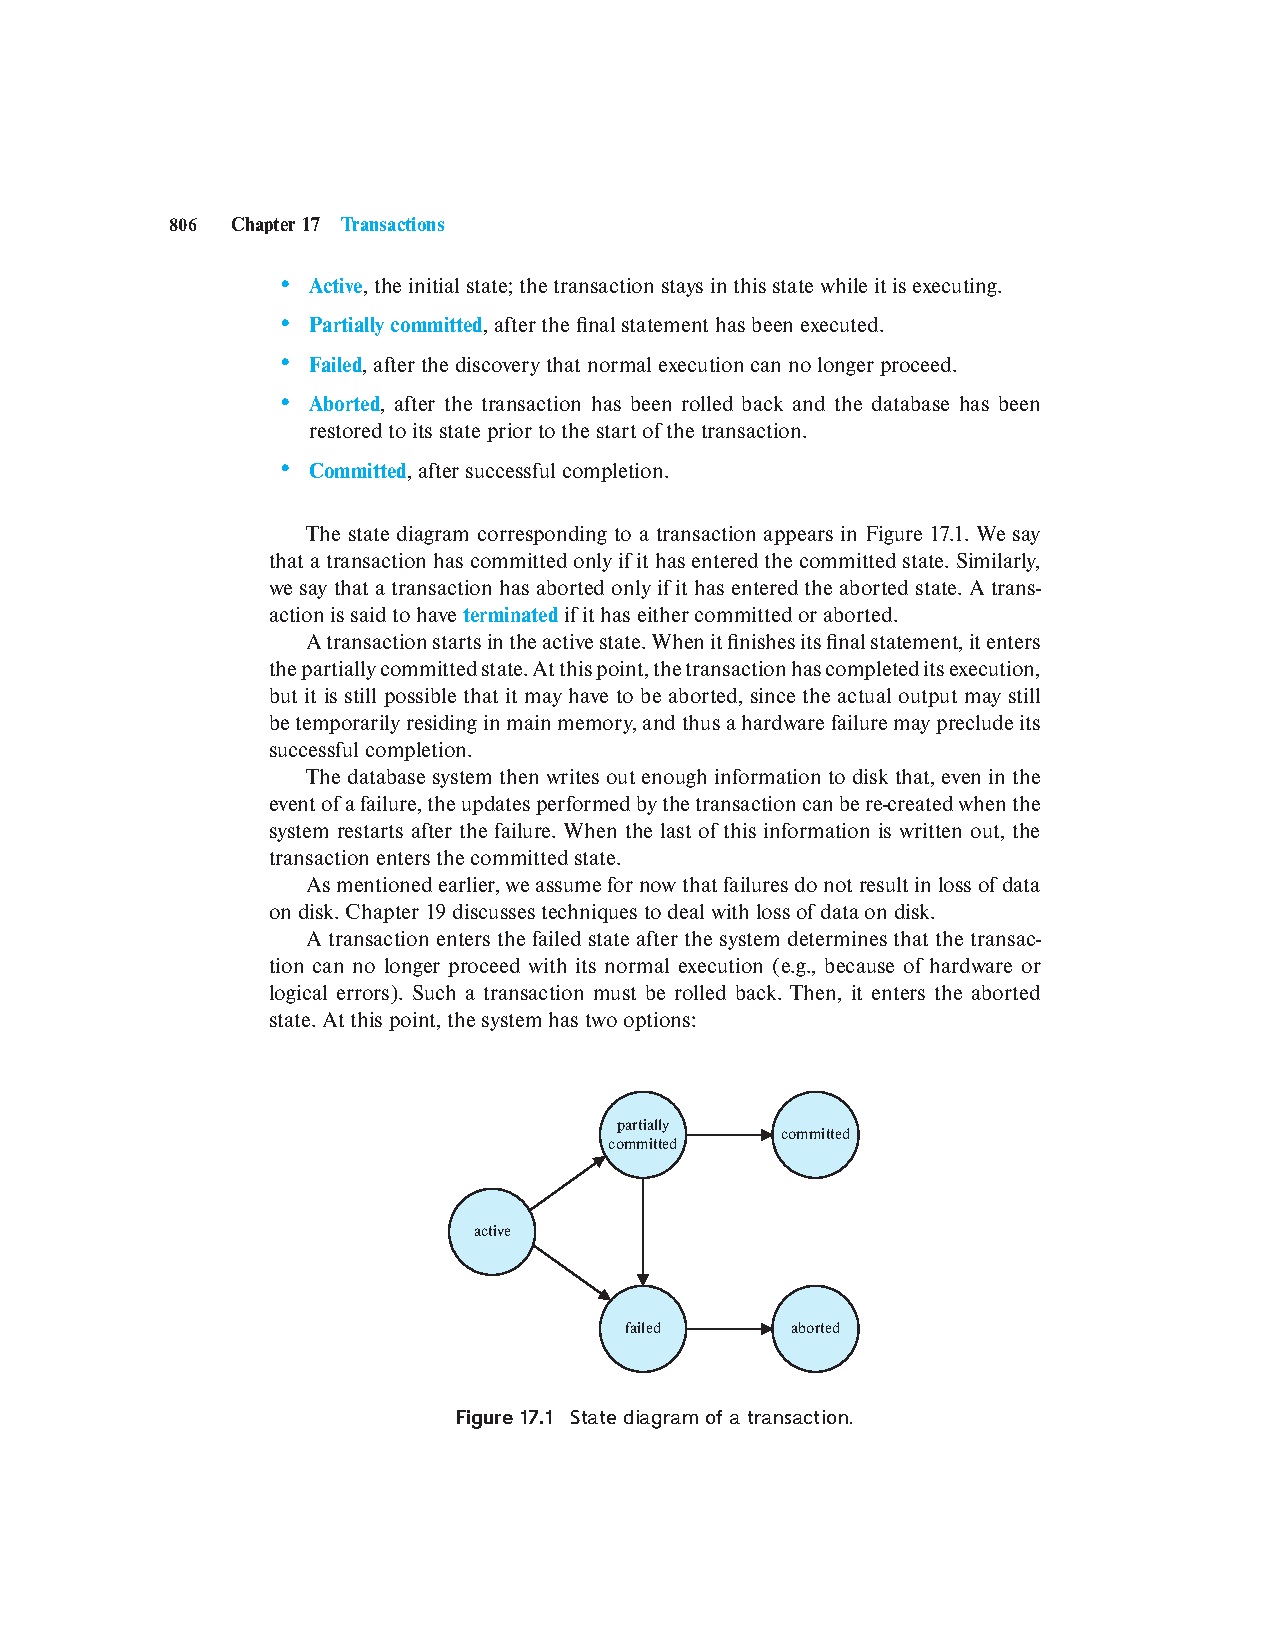
\includegraphics[width=\textwidth, trim={5cm 3cm 5cm 18cm}, clip]{figures/p835_stages.pdf}
\end{frame}

\begin{frame}{Concurrent Executions}
    \footnotesize
    Multiple transactions are allowed to run concurrently in the system.  Advantages are:
        \begin{itemize}
            \item Increased processor and disk utilization, leading to better transaction throughput. \\        \quad e.g., one transaction can be using the CPU while another is reading from or writing to    the disk
            \item Reduced average response time for transactions: short transactions need not wait behind long ones.
            \item Better resource utilization
        \end{itemize}

    Concurrency control schemes – mechanisms to achieve isolation:
        \begin{itemize}
            \item That is, to control the interaction among the concurrent transactions in order to prevent them from destroying the consistency of the database.
            \item They are studied in Chapter 15, after studying notion of correctness of concurrent executions.
        \end{itemize}

\end{frame}

\begin{frame}{Schedules}
    \textbf{Schedule} – a sequences of instructions that specify the chronological order in which instructions of concurrent transactions are executed:
        \begin{itemize}
            \item A schedule for a set of transactions must consist of all instructions of those transactions
            \item Must preserve the order in which the instructions appear in each individual transaction.
        \end{itemize}

    A transaction that successfully completes its execution will have a commit instructions as the last statement.
        \begin{itemize}
            \item By default transaction assumed to execute commit instruction as its last step.
        \end{itemize}

    A transaction that fails to successfully complete its execution will have an abort instruction as the last statement.
\end{frame}

\begin{frame}{Schedules 1}

    Let $T_1$ transfer \$50 from A to B, and $T_2$ transfer 10\% of the balance from A to B.
    A \textbf{serial} schedule in which $T_1$ is followed by $T_2$:
    \begin{center}
        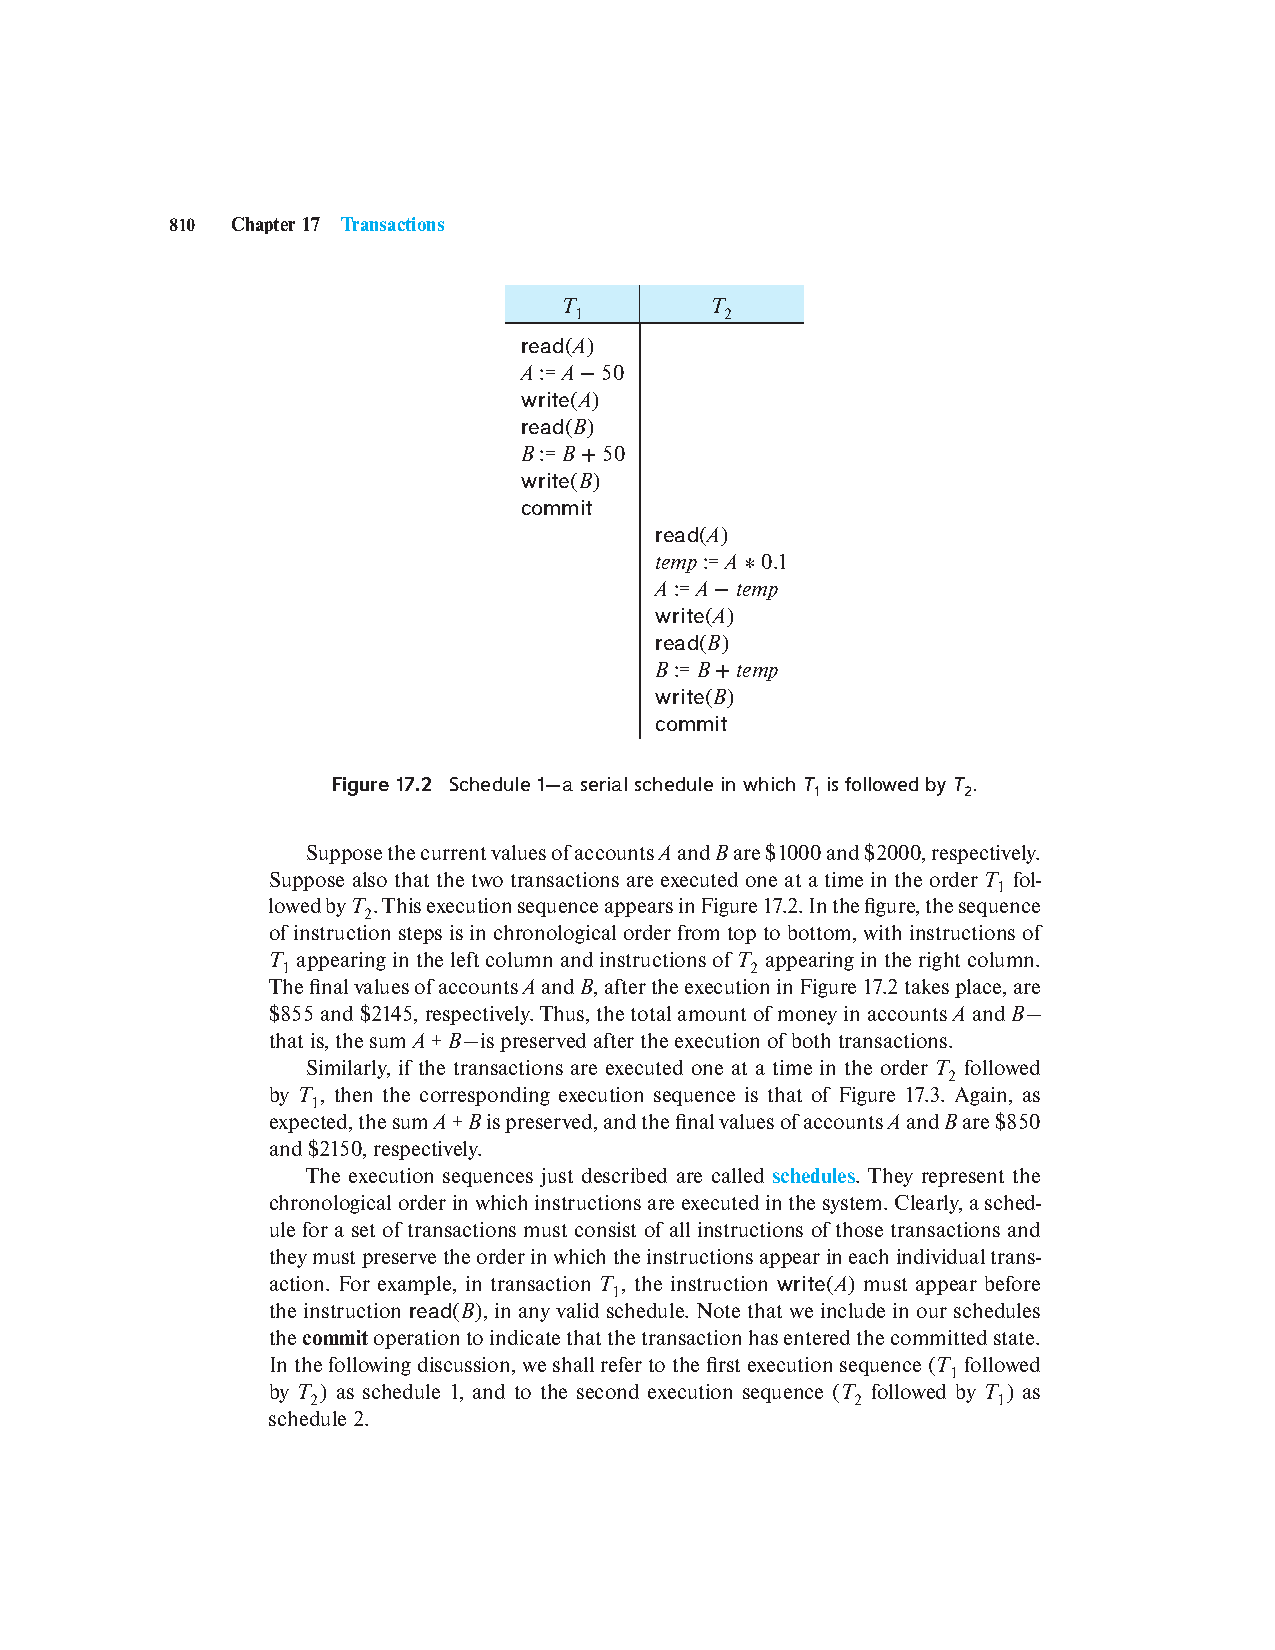
\includegraphics[width=\textwidth, trim={2cm 14cm 2cm 4cm}, clip]{figures/p839_schedule1}
    \end{center}

\end{frame}

\begin{frame}{Schedules 2}

    A serial schedule where $T_2$ is followed by $T_1$:
    \begin{center}
        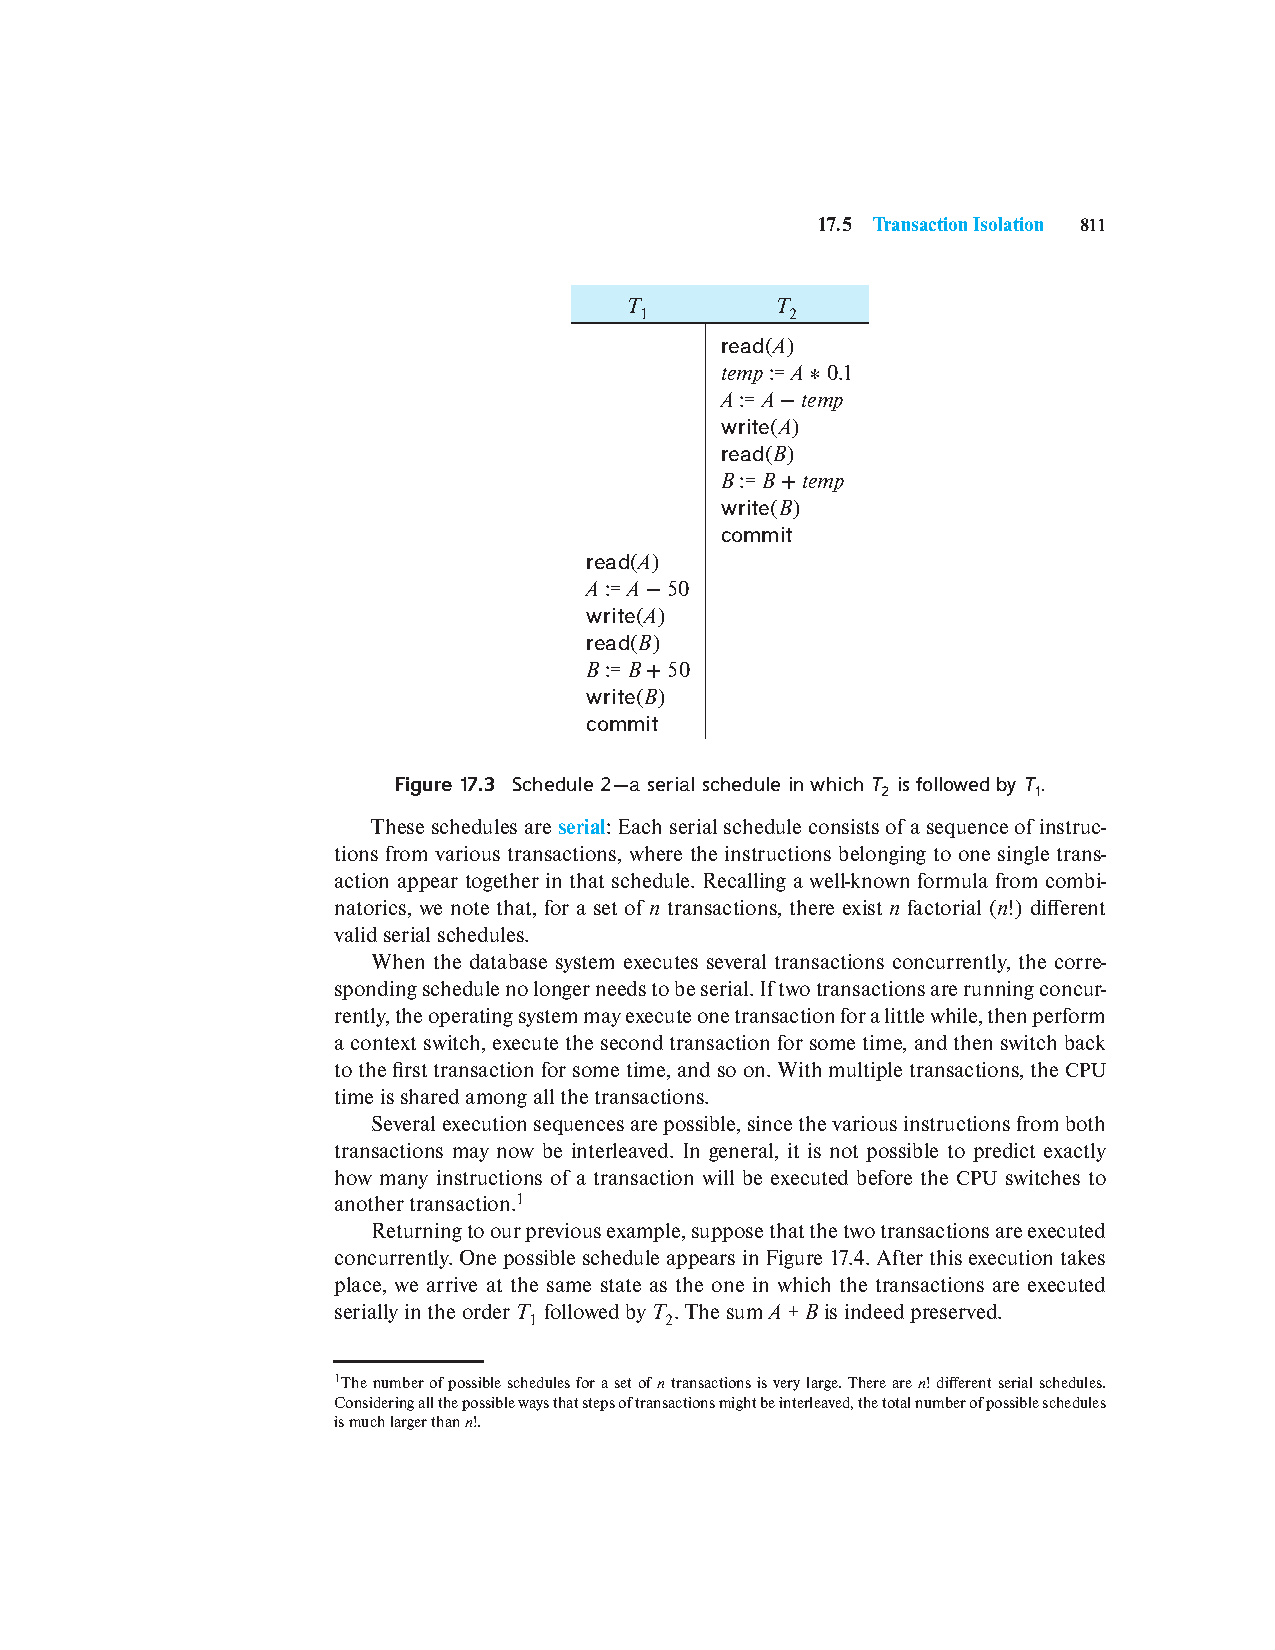
\includegraphics[width=\textwidth, trim={2cm 14.25cm 2cm 4cm}, clip]{figures/p840_schedule2}
    \end{center}

\end{frame}

\begin{frame}{Schedules 3}

    Let $T_1$ and $T_2$ be the transactions defined previously. The following schedule is not a serial schedule, but it is \textbf{equivalent} to Schedule 1:
    \begin{center}
        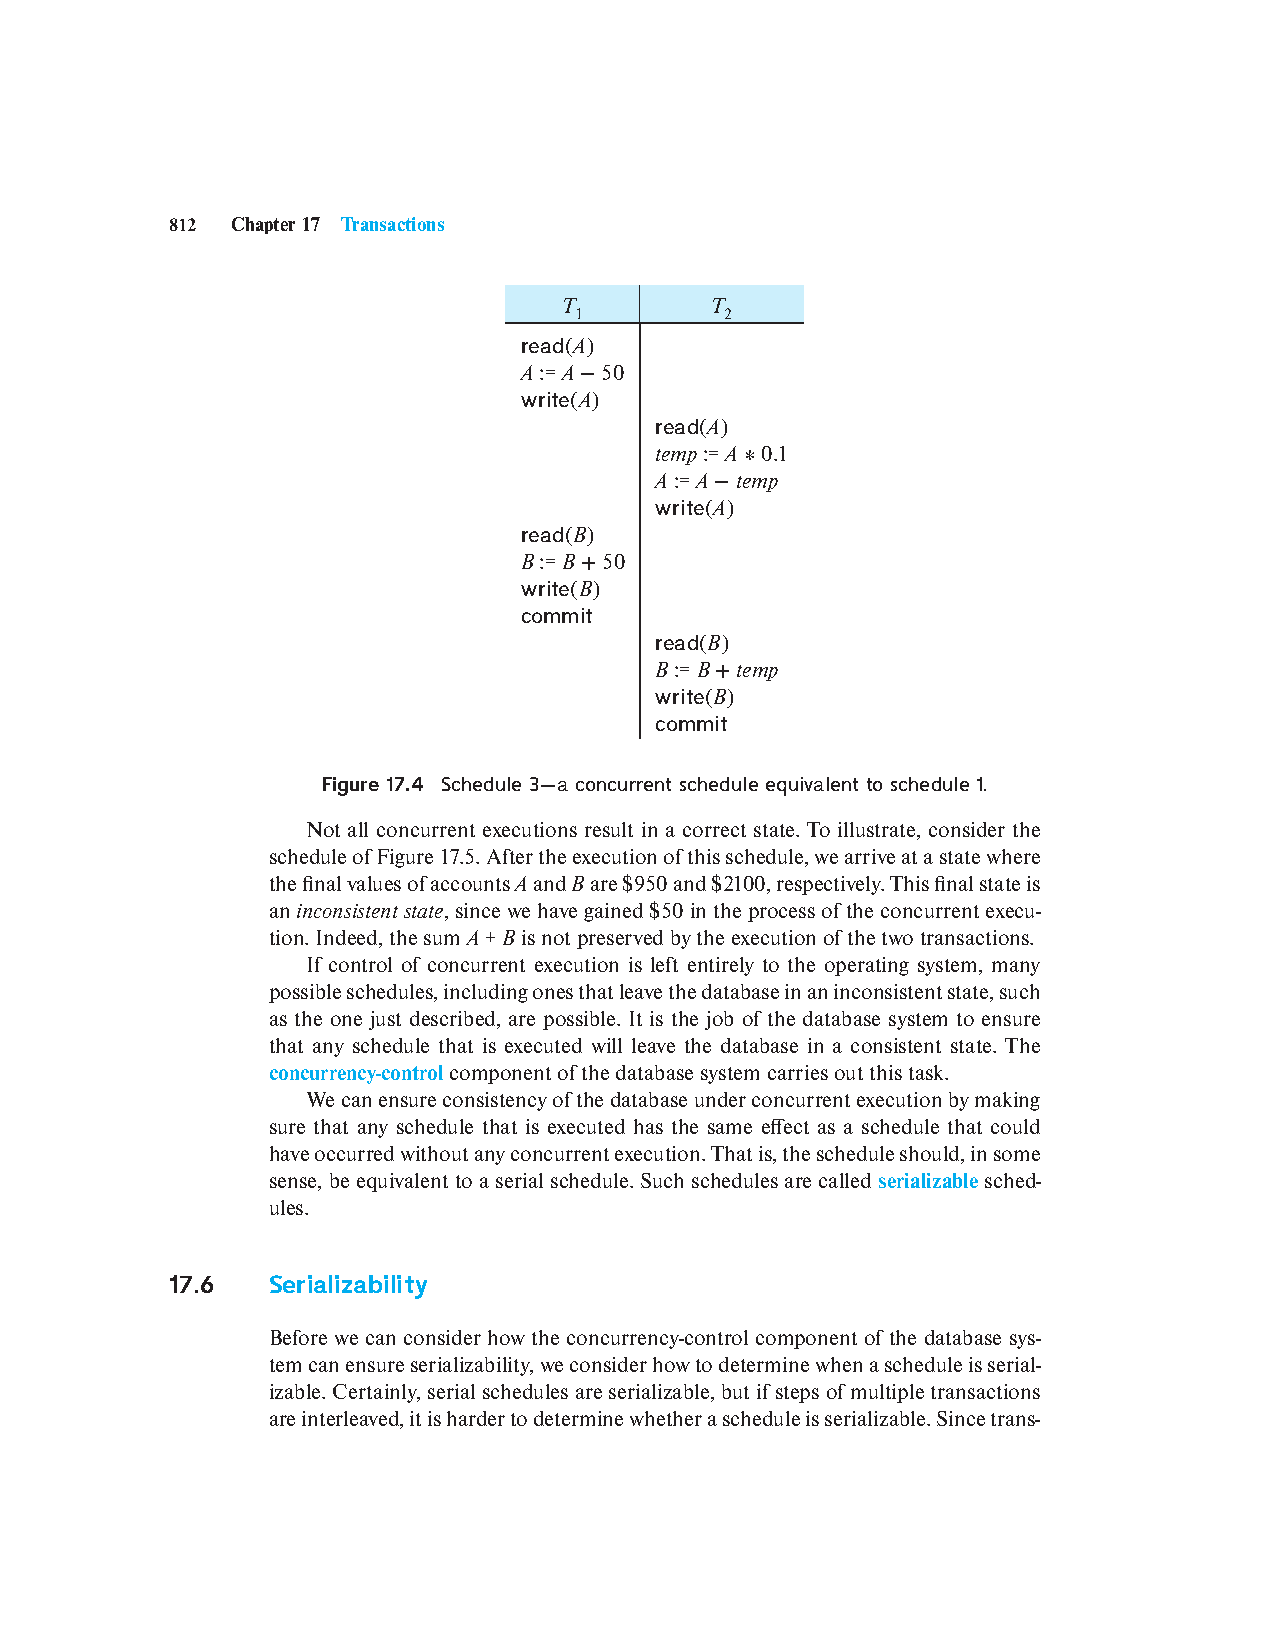
\includegraphics[width=\textwidth, trim={2cm 14.25cm 2cm 4cm}, clip]{figures/p841_schedule3}
    \end{center}
    In Schedules 1, 2 and 3, the sum A + B is preserved.

\end{frame}

\begin{frame}{Schedules 4}

    The following concurrent schedule does not preserve the value of (A + B ).
    \begin{center}
        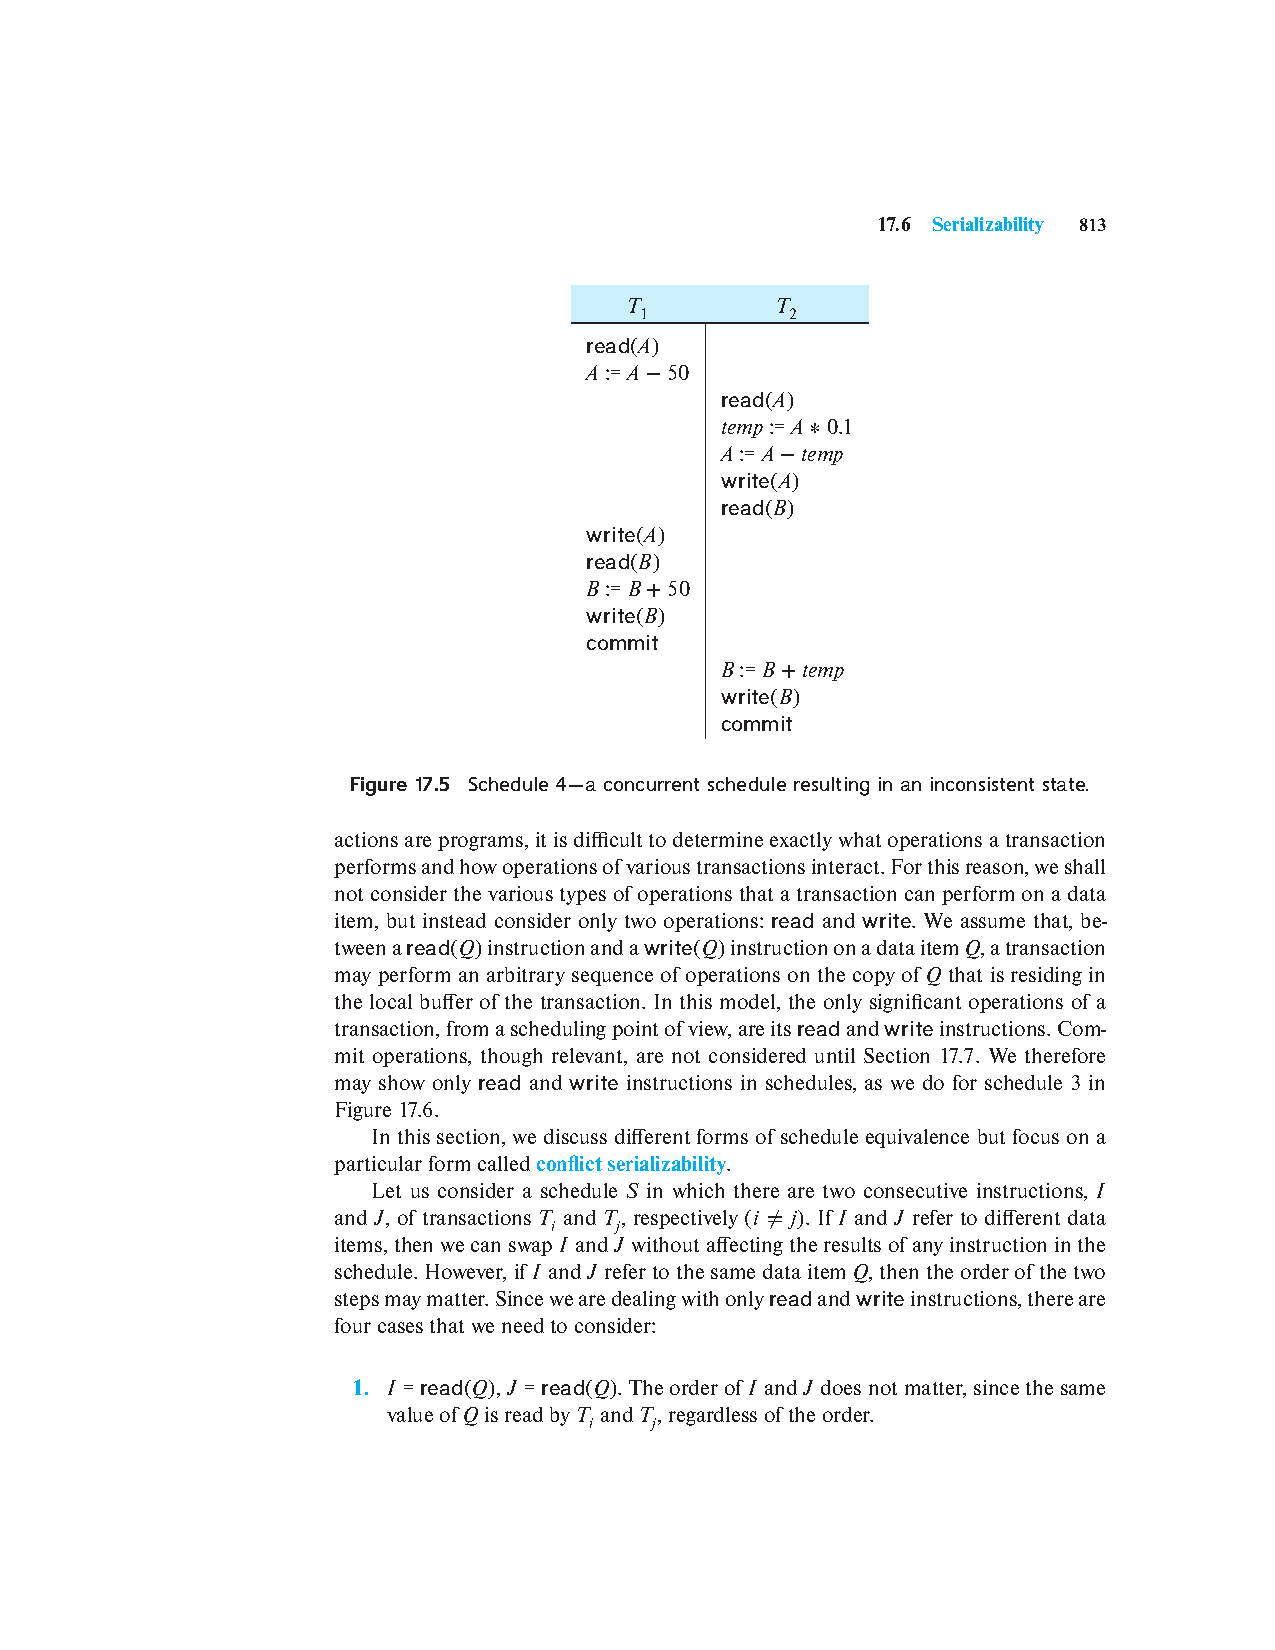
\includegraphics[width=\textwidth, trim={2cm 14.25cm 2cm 4cm}, clip]{figures/p842_schedule4}
    \end{center}

\end{frame}


\section{Serializability}

\begin{frame}{Serializability}

    \begin{itemize}
        \item If it is equivalent to a serial execution and ensures the database remains consistent.
        \item Basic Assumption – Each transaction preserves database consistency.
        \item Thus, serial execution of a set of transactions preserves database consistency.
        \item A (possibly concurrent) schedule is serializable if it is equivalent to a serial schedule. Different forms of schedule equivalence give rise to the notions of:
            \begin{enumerate}
                \item \textit{conflict serializability}
                \item \textit{view serializability}
            \end{enumerate}
    \end{itemize}

\end{frame}

\begin{frame}{\textit{Simplified view of transactions}}
    \begin{itemize}
        \item We ignore operations other than read and write instructions.
        \item We assume that transactions may perform arbitrary computations on data in local buffers in between reads and writes.
        \item Our simplified schedules consist of only read and write instructions.
    \end{itemize}
\end{frame}

\begin{frame}{Conflicting Instructions}
    \begin{itemize}
        \item Instructions $l_i$ and $l_j$ of transactions $T_i$ and $T_j$ respectively, conflict if and only if there exists some item $Q$ accessed by both $l_i$ and $l_j$, and at least one of these instructions wrote $Q$.
            \begin{enumerate}
                \item $l_i$ = \texttt{read(Q)}, $l_j$ = \texttt{read(Q)}. $l_i$ and $l_j$ don't conflict.
                \item $l_i$ = \texttt{write(Q)}, $l_j$ = \texttt{read(Q)}. They conflict.
                \item $l_i$ = \texttt{read(Q)}, $l_j$ = \texttt{write(Q)}. They conflict.
                \item $l_i$ = \texttt{write(Q)}, $l_j$ = \texttt{write(Q)}. They conflict.
            \end{enumerate}

        \item Intuitively, a conflict between $l_i$ and $l_j$ forces a (logical) temporal order between them.
            \begin{itemize}
                \item If $l_i$ and $l_j$ are consecutive in a schedule and they do not conflict, their results would remain the same even if they had been interchanged in the schedule.
            \end{itemize}

    \end{itemize}
\end{frame}

\begin{frame}{Conflict Serializability}
    \begin{itemize}
        \item Based on detecting conflicts in transaction operations.
        \item Conflicts arise when two transactions access the same data item and at least one is a write operation.
    \end{itemize}
\end{frame}

\begin{frame}{Conflict Serializability (Cont.)}
    \begin{itemize}
        \item If a schedule S can be transformed into a schedule S' by a series of swaps of non-conflicting instructions, we say that S and S' are conflict equivalent.
        \item We say that a schedule S is conflict serializable if it is conflict equivalent to a serial schedule.
    \end{itemize}
\end{frame}

\begin{frame}{Conflict Serializability (Cont.)}
    \begin{itemize}
        \item Schedule 3 can be transformed into Schedule 6, a serial schedule where $T2$ follows $T1$, by series of swaps of non-conflicting instructions. Therefore Schedule 3 is conflict serializable.
    \end{itemize}
    \centering
    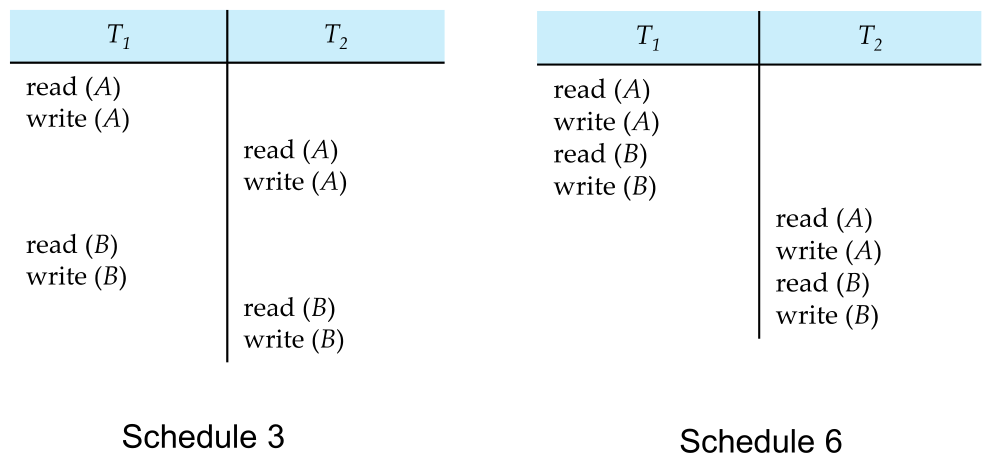
\includegraphics[width=.9\textwidth]{figures/conflict_ser1}
\end{frame}

\begin{frame}{Conflict Serializability (Cont.)}
    \begin{itemize}
        \item Example of a schedule that is not conflict serializable:
    \end{itemize}
    \centering
    
\includegraphics[width=.9\textwidth]{figures/conflict_ser2}
    \begin{itemize}
        \item We are unable to swap instructions in the above schedule to obtain either the serial schedule $< T_3, T_4 >$, or the serial schedule $< T_4, T_3 >$.
    \end{itemize}
\end{frame}

\begin{frame}{View Serializability}
    \begin{itemize}
        \item Considers the final outcome of transactions, not just conflicts.
        \item More general but harder to test than conflict serializability.
    \end{itemize}
\end{frame}

\begin{frame}{View Serializability (Cont.)}

    \begin{itemize}
        \item Let S and S' be two schedules with the same set of transactions. S and S' are view equivalent if the following three conditions are met, for each data item Q,
            \begin{enumerate}
                \item If in schedule S, transaction $T_i$ reads the initial value of Q, then in schedule S' also transaction $T_i$ must read the initial value of Q.
                \item If in schedule S transaction $T_i$ executes \texttt{read(Q)}, and that value was produced by transaction $T_j$ (if any), then in schedule S' also transaction $T_i$ must read the value of Q that was produced by the same \texttt{write(Q)} operation of transaction $T_j$.
                \item The transaction (if any) that performs the final \texttt{write(Q)} operation in schedule S must also perform the final \texttt{write(Q)} operation in schedule S'.
            \end{enumerate}
        \item As can be seen, view equivalence is also based purely on \textbf{reads} and \textbf{writes} alone.
    \end{itemize}

\end{frame}

\begin{frame}{View Serializability (Cont.)}
    \begin{itemize}
        \item A schedule S is view serializable if it is view equivalent to a serial schedule.
        \item Every conflict serializable schedule is also view serializable.
        \item Below is a schedule which is view-serializable but not conflict serializable.
            
\includegraphics[width=.9\textwidth]{figures/view_ser1}
        \item What serial schedule is above equivalent to?
        \item Every view serializable schedule that is not conflict serializable has blind writes.
    \end{itemize}
\end{frame}

\begin{frame}{Other Notions of Serializability}
    \begin{itemize}
        \item The schedule below produces same outcome as the serial schedule $< T_1, T_5 >$, yet is not conflict equivalent or view equivalent to it.
            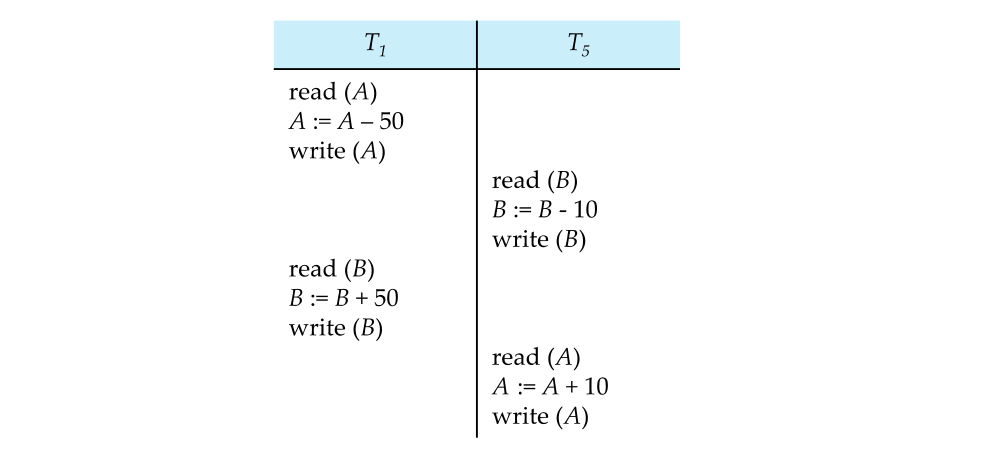
\includegraphics[width=.9\textwidth]{figures/view_ser2}
        \item Determining such equivalence requires analysis of operations other than read and write.
    \end{itemize}
\end{frame}

\section{Testing for Serializability}

\begin{frame}{Testing for Serializability}
    \begin{itemize}
        \item Consider some schedule of a set of transactions $T_1, T_2, \ldots, T_n$
        \item \textbf{Precedence graph} — a direct graph where the vertices are the transactions (names).
        \item We draw an arc from $T_i$ to $T_j$ if the two transaction conflict, and $T_i$ accessed the data item on which the conflict arose earlier.
        \item We may label the arc by the item that was accessed.
    \end{itemize}
\end{frame}

\begin{frame}{Precedence Graphs}
    \begin{itemize}
        \item Used to test for conflict serializability.
        \item Graph cycles indicate non-serializable schedules.
        \item Example 1
            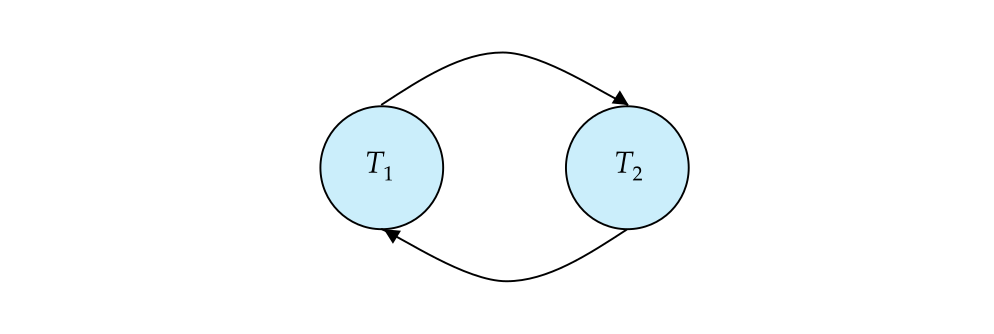
\includegraphics[width=.9\textwidth]{figures/graph1}
    \end{itemize}
\end{frame}

\begin{frame}{Test for Conflict Serializability}
    \begin{itemize}
        \item A schedule is conflict serializable if and only if its precedence graph is acyclic.
        \item Cycle-detection algorithms exist which take order $n^2$ time, where $n$ is the number of vertices in the graph.
        \item If precedence graph is acyclic, the serializability order can be obtained by a \textit{topological sorting} of the graph.
    \end{itemize}
\end{frame}

\begin{frame}{Test for Conflict Serializability (Cont.)}

    \centering
    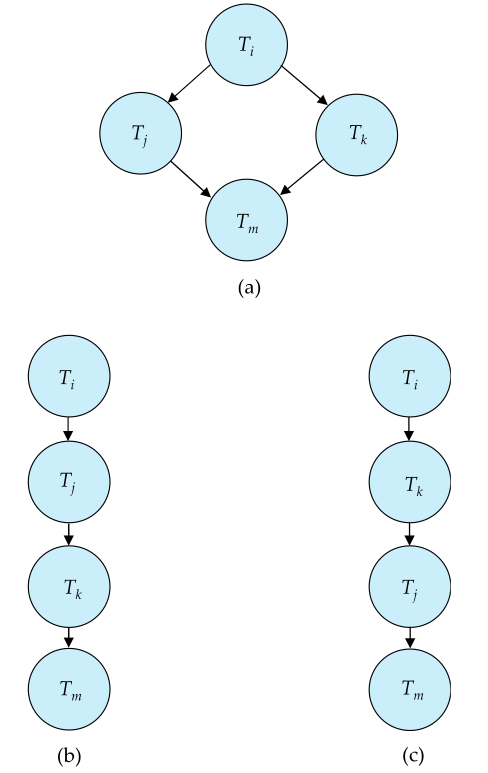
\includegraphics[width=.4\textwidth]{figures/graph2}

\end{frame}

\begin{frame}{Test for View Serializability}

    \begin{itemize}
        \item The precedence graph test for conflict serializability cannot be used directly to test for view serializability.
            \begin{itemize}
                \item Extension to test for view serializability has cost exponential in the size of the precedence graph.
            \end{itemize}
        \item The problem of checking if a schedule is view serializable falls in the class of NP-complete problems.
            \begin{itemize}
                \item Thus. existence of an efficient algorithm is extremely unlikely.
            \end{itemize}
        \item However practical algorithms that just check some \textbf{sufficient conditions} for view serializability can still be used.
    \end{itemize}

\end{frame}

\begin{frame}{Recoverable Schedules}

    Need to address the effect of transaction failures on concurrently running transactions.
    \begin{itemize}
        \item \textbf{Recoverable schedule} — if a transaction $T_j$ reads a data item previously written by a transaction $T_i$, then the commit operation of $T_i$ appears before the commit operation of $T_j$.
        \item The following schedule (Schedule 11) is not recoverable:
            
\includegraphics[width=.9\textwidth]{figures/schedule1}
        \item If $T_8$ should abort, $T_9$ would have read (and possibly shown to the user) an inconsistent database state. Hence, database must ensure that schedules are recoverable.
    \end{itemize}

\end{frame}

\begin{frame}{Cascading Rollbacks}

    \begin{itemize}
        \item \textbf{Cascading rollback} – a single transaction failure leads to a series of transaction rollbacks. Consider the following schedule where none of the transactions has yet committed (so the schedule is recoverable)

            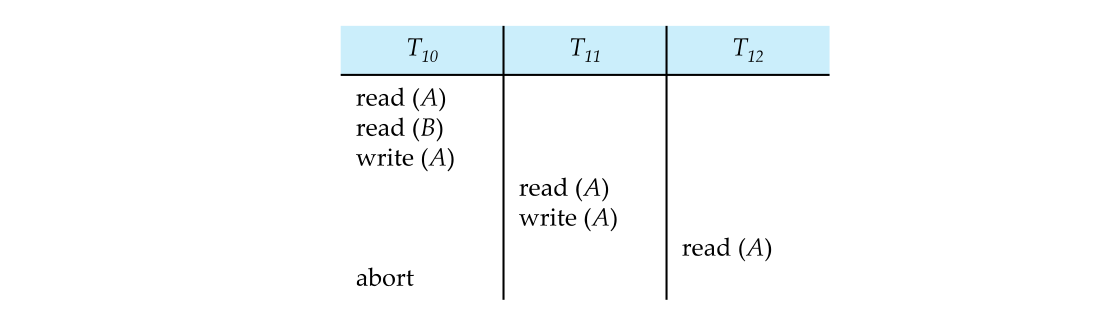
\includegraphics[width=.9\textwidth]{figures/cascade1}

        If $T_{10}$ fails, $T_{11}$ and $T_{12}$ must also be rolled back.

        \item Can lead to the undoing of a significant amount of work.
    \end{itemize}

\end{frame}

\begin{frame}{Cascadeless Schedules}

    \begin{itemize}
        \item \textbf{Cascadeless schedules} — cascading rollbacks cannot occur:
            \begin{itemize}
                \item For each pair of transactions $T_i$ and $T_j$ such that $T_j$ reads a data item previously written by $T_i$, the commit operation of $T_i$ appears before the read operation of $T_j$.
            \end{itemize}
        \item Every cascadeless schedule is also recoverable.
        \item It is desirable to restrict the schedules to those that are cascadeless.
    \end{itemize}

\end{frame}

\section{Concurrency Control}

\begin{frame}{Concurrency Control}

    \begin{itemize}
        \item A database must provide a mechanism that will ensure that all possible schedules are:
            \begin{itemize}
                \item either conflict or view serializable, and
                \item are recoverable and preferably cascadeless.
            \end{itemize}
        \item A policy in which only one transaction can execute at a time generates serial schedules, but provides a poor degree of concurrency,
            \begin{itemize}
                \item Are serial schedules recoverable/cascadeless?
            \end{itemize}
        \item Testing a schedule for serializability after it has executed is a little too late!
        \item \textbf{Goal} – to develop concurrency control protocols that will assure serializability.
    \end{itemize}

\end{frame}

\begin{frame}{Concurrency Control (Cont.)}

    \begin{itemize}
        \item Schedules must be conflict or view serializable, and recoverable, for the sake of database consistency, and preferably cascadeless.
        \item A policy in which only one transaction can execute at a time generates serial schedules, but provides a poor degree of concurrency.
        \item Concurrency-control schemes tradeoff between the amount of concurrency they allow and the amount of overhead that they incur.
        \item Some schemes allow only conflict-serializable schedules to be generated, while others allow view-serializable schedules that are not conflict-serializable.
    \end{itemize}

\end{frame}

\begin{frame}{Concurrency Control vs. Serializability Tests}

    \begin{itemize}
        \item Concurrency-control protocols allow concurrent schedules, but ensure that the schedules are conflict/view serializable, and are recoverable and cascadeless.
        \item Concurrency control protocols (generally) do not examine the precedence graph as it is being created,
            \begin{itemize}
                \item Instead a protocol imposes a discipline that avoids non-serializable schedules.
                \item We study such protocols in Chapter 16.
            \end{itemize}
        \item Different concurrency control protocols provide different tradeoffs between the amount of concurrency they allow and the amount of overhead that they incur.
        \item Tests for serializability help us understand why a concurrency control protocol is correct.
    \end{itemize}

\end{frame}

\begin{frame}{Weak Levels of Consistency}

    \begin{itemize}
        \item Some applications are willing to live with weak levels of consistency, allowing schedules that are not serializable,
            \begin{itemize}
                \item E.g., a read-only transaction that wants to get an approximate total balance of all accounts.
                \item E.g., database statistics computed for query optimization can be approximate (why?).
                \item Such transactions need not be serializable with respect to other transactions.
            \end{itemize}
        \item Tradeoff accuracy for performance.
    \end{itemize}

\end{frame}

\begin{frame}{Levels of Consistency in SQL-92}

    \begin{itemize}
        \item \textbf{Serializable} — default
        \item \textbf{Repeatable read} — only committed records to be read.
            \begin{itemize}
                \item Repeated reads of same record must return same value.
                \item However, a transaction may not be serializable – it may find some records inserted by a transaction but not find others.
            \end{itemize}
        \item \textbf{Read committed} — only committed records can be read.
            \begin{itemize}
                \item Successive reads of record may return different (but committed) values.
            \end{itemize}
        \item \textbf{Read uncommitted} — even uncommitted records may be read.
    \end{itemize}

\end{frame}

\begin{frame}{Levels of Consistency}

    \begin{itemize}
        \item Lower degrees of consistency useful for gathering approximate information about the database.
        \item Warning: some database systems do not ensure serializable schedules by default.
        \item E.g., Oracle (and PostgreSQL prior to version 9) by default support a level of consistency called snapshot isolation (not part of the SQL standard).
    \end{itemize}

\end{frame}

\section{Transaction Definition in SQL}

\begin{frame}[fragile]{Transaction Definition in SQL}
    \begin{itemize}
        \item Transactions begin implicitly.
        \item End with COMMIT or ROLLBACK.
        \item Example in SQL:
    \end{itemize}
    \begin{minted}
    [tabsize=4, obeytabs, frame=lines, framesep=2mm, baselinestretch=1.2, bgcolor=LightGray, fontsize=\scriptsize]{sql}

    BEGIN TRANSACTION;
    UPDATE accounts SET balance = balance - 50 WHERE id = 'A';
    UPDATE accounts SET balance = balance + 50 WHERE id = 'B';
    COMMIT;

    \end{minted}
\end{frame}

\begin{frame}{Transaction Definition in SQL}
    \begin{itemize}
        \item In almost all database systems, by default, every SQL statement also commits implicitly if it executes successfully,
            \begin{itemize}
                \item Implicit commit can be turned off by a database directive
                    \begin{itemize}
                        \item E.g., in JDBC -- \texttt{connection.setAutoCommit(false);}
                    \end{itemize}

            \end{itemize}
        \item Isolation level can be set at database level
        \item Isolation level can be changed at start of transaction
            \begin{itemize}
                \item E.g. In SQL set transaction isolation level serializable
                \item E.g. in JDBC -- \\
                    \begin{scriptsize}
                \texttt{connection.setTransactionIsolation(} \\
                \quad \texttt{Connection.TRANSACTION\_SERIALIZABLE} \\
                \texttt{);}
                    \end{scriptsize}

            \end{itemize}
    \end{itemize}
\end{frame}

\begin{frame}{Implementation of Isolation Levels}
    Overview
    \begin{itemize}
        \item Locking
            \begin{itemize}
                \item Lock on whole database vs lock on items.
                \item How long to hold lock?
                \item Shared vs exclusive locks.
            \end{itemize}
        \item Timestamps
            \begin{itemize}
                \item Transaction timestamp assigned e.g. when a transaction begins
                \item Data items store two timestamps:
                    \begin{itemize}
                        \item Read timestamp.
                        \item Write timestamp.
                    \end{itemize}
                \item Timestamps are used to detect out of order accesses.
            \end{itemize}
        \item Multiple versions of each data item,
            \begin{itemize}
             \item Allow transactions to read from a ``snapshot'' of the database.
            \end{itemize}
    \end{itemize}
\end{frame}



\section{Conclusion}

\begin{frame}{Conclusion}
    \begin{itemize}
        \item Transactions are essential for database consistency.
        \item Proper isolation and concurrency control are critical.
        \item Advanced techniques like serializability testing ensure reliable performance.
    \end{itemize}
\end{frame}









\begin{frame}{}
\end{frame}

% \begin{frame}[fragile]{}
%     \begin{minted}
%     [tabsize=4, obeytabs, frame=lines, framesep=2mm, baselinestretch=1.2, bgcolor=LightGray, fontsize=\scriptsize]{sql}
%     \end{minted}
% \end{frame}

\begin{frame}{}
     \centering
     \Huge End of Chapter 7.
\end{frame}

\section*{Takeaways}

% Tim Duncan's Top 5 Fundamental Takeaways of the Today's Class
\begin{frame}{TDT5FTOTTC}
    \centering
    
\includegraphics[width=0.75\textwidth]{figures/tim.png}
\end{frame}

\begin{frame}{Top 5 Fundamental Takeaways}
    \small
    \begin{enumerate} \pause
        \item[5] Good relational design reduces redundancy and avoids update anomalies by ensuring data is stored without unnecessary repetition or nulls. \pause

        \item[4] Lossless and dependency-preserving decomposition ensures that a schema can be split without losing data or making constraint enforcement inefficient. \pause

        \item[3] Functional dependencies and normal forms guide how to structure schemas to eliminate redundancy while preserving meaningful data relationships. \pause

        \item[2] Canonical covers provide a minimal, simplified set of functional dependencies that retain the original semantics for efficient constraint checking. \pause

        \item[1] Fourth Normal Form (4NF) extends normalization to eliminate redundancy caused by multivalued dependencies, ensuring cleaner data representation.
    \end{enumerate}
\end{frame}

\begin{frame}{Database System Concepts}
    \centering
    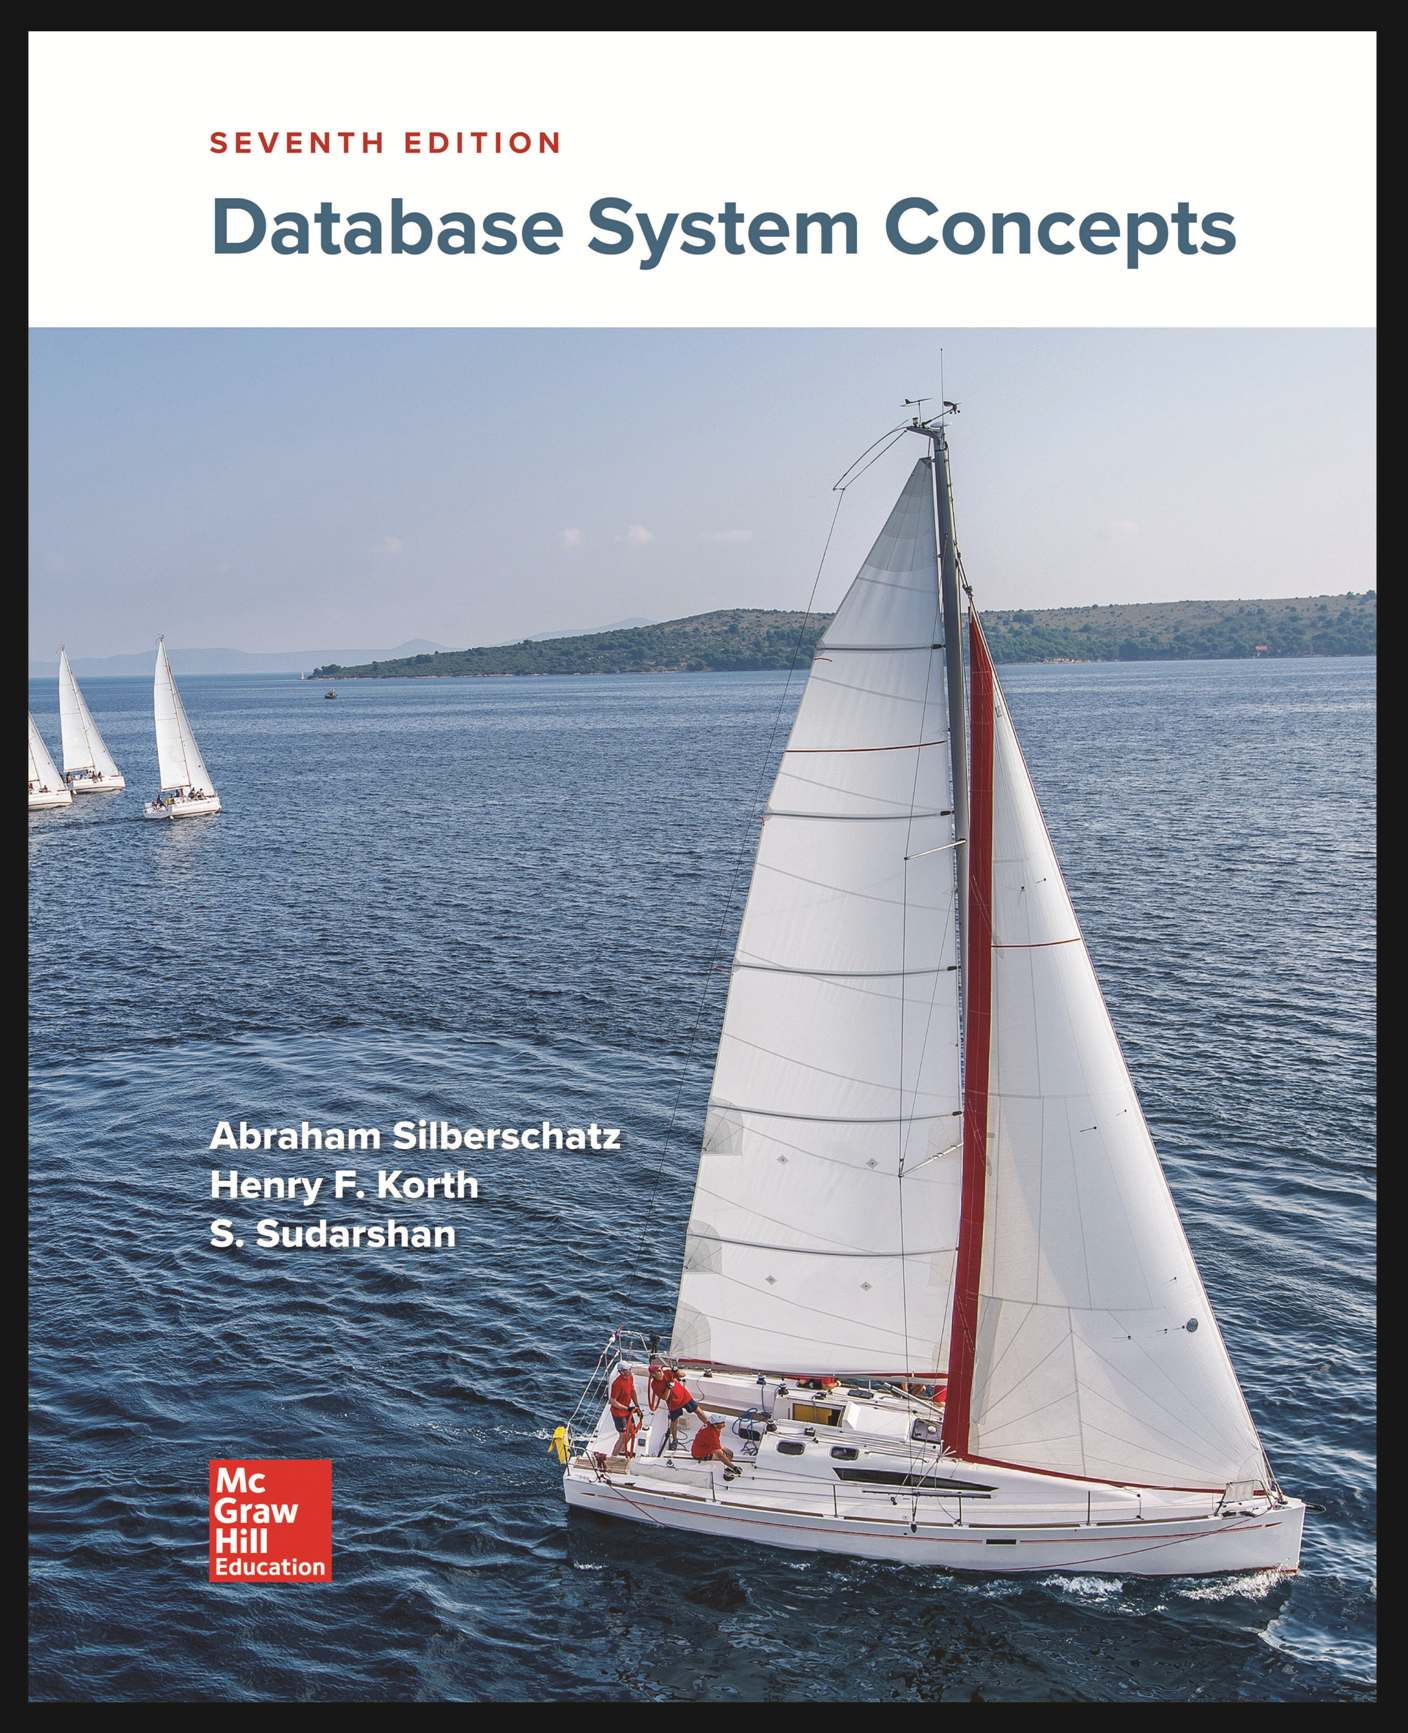
\includegraphics[width=0.5\textwidth]{figures/book_cover.jpg} \\
    \vspace{5mm}
    {
        \tiny
        Content has been extracted from \textit{Database System Concepts}, Seventh Edition, by Silberschatz, Korth and Sudarshan. Mc Graw Hill Education. 2019.\\
        Visit \url{https://db-book.com/}.\\
    }
\end{frame}

\end{document}
